%
% halbkreiskontur.tex
%
% (c) 2026 Damien Flury, OST Ostschweizer Fachhochschule
%
\begin{figure}
\centering
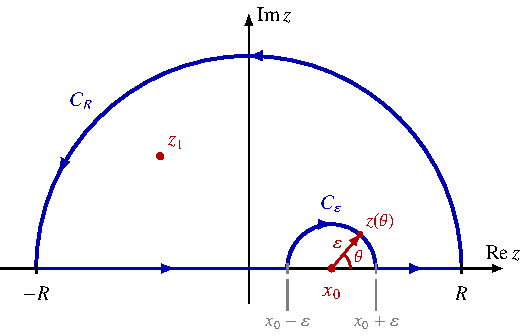
\includegraphics{papers/hauptwert/images/halbkreiskontur.pdf}
\caption{Halbkreiskontur zur Berechnung von Hauptwerten.
Die Kontur wird im positiven Sinn durchlaufen und besteht aus den beiden
Strecken auf der reellen Achse, der Einbuchtung $C_\varepsilon$ oberhalb der
Polstelle $x_0$ und dem grossen Halbkreis $C_R$.
Die Einbuchtung schliesst $x_0$ aus dem umlaufenen Gebiet aus und wird
dabei im negativen Sinn durchlaufen;
eingeschlossen wird nur der Pol $z_1$ in der oberen Halbebene.
\label{hauptwert:figure:halbkreiskontur}}
\end{figure}
